\section{Algoritmen}

\begin{figure}[hbtp]
  \centering
  \resizebox {\textwidth} {!} {
    \begin{tikzpicture}[scale=1.5]
      % grid
      \draw[very thin,color=lightgray] (0,0) grid (7,7);
      \draw [<->,thick] (0,7) node (yaxis) [left] {Y} |- (7,0) node (xaxis) [right] {X};
      
      \circle[1,2,1.5,1]
      \circle[2,4.5,2,1]    
      \circle[3,5.5,3,1]
      \circle[4,5,5.5,1]
      
    \end{tikzpicture}
  }
  \label{fig:voorbeeld_opgave}
  \caption{Een voorbeeld opgave}
\end{figure}


\subsection{Snijpunt van twee cirkels berekenen}
\label{sec:snijpunt}

\subsubsection{Algoritme}
\begin{algorithm}[H]
  \SetAlgoLined
  \KwIn{twee cirkels, $c$ en $c'$ met resp middelpunten $p_{1}, p_{2}$ en stralen $r_{1}, r_{2}$}
  \KwOut{waar als en slechts als de twee cirkels snijden}
  \SetKwProg{Fn}{Procedure}{:}{end}
  \Fn{intersect($c$,$c'$)}{
    d $\leftarrow \lVert p_2 - p_1\rVert $\\
    \eIf{($d \leq r_1 + r_2) \land (d \geq abs (r_1 - r_2))$}{
      \Return{true}
    }{
      \Return{false}
    }
  }

  \caption{Nagaan of twee cirkels snijden}
\end{algorithm}

\begin{algorithm}[H]
  \SetAlgoLined
  \KwIn{twee cirkels, $c$ en $c'$ met resp. middelpunten $p_{1} = (x_1,y_1), p_{2} = (x_2,y_2)$ en stralen $r_{1}, r_{2}$}
  \KwOut{geen, of twee snijpunten van de twee cirkels (die dan identiek zijn)}
  \SetKwProg{Fn}{Procedure}{:}{end}
  \Fn{intersections($c$,$c'$)}{
    \eIf{$intersect(c, c') \land c1 \neq c2$}{
      $d \leftarrow \lVert p_2 - p_1\rVert $ \\
      $\alpha \leftarrow \frac{r_1^2 -r_2^2}{2d^2}$\\
      $s \leftarrow \frac{x_1+x_2}{2} + \alpha(x_2-x_1)$\\
      $t \leftarrow \frac{y_1+y_2}{2} + \alpha(y_2-y_1)$\\

      $\delta \leftarrow \frac{1}{4}  \sqrt { (d+r_1+r_2)(d+r_1-r_2)(d-r_1+r_2)(r_1+r_2-d)}$\\
      $x_1' \leftarrow s + 2\delta\frac{y_1-y_2}{d^2}$\\
      $x_2' \leftarrow s - 2\delta\frac{y_1-y_2}{d^2}$\\
      $y_1' \leftarrow t - 2\delta\frac{x_1-x_2}{d^2}$\\
      $y_2' \leftarrow t + 2\delta\frac{x_1-x_2}{d^2}$\\
      \Return{$\left\{(x_1',y_1'),(x_2',y_2')\right\}$}
    }{
      \Return{$\varnothing$}
    }
  }
  \caption{Snijpunten van twee cirkels berekenen}
\end{algorithm}

\subsubsection{Correctheidsbewijs}
\subsubsection{Complexiteit}


\subsection{Na\"ief}
\label{sec:naief}

\subsubsection{Algoritme}

\begin{algorithm}[H]
  \SetAlgoLined
  \KwIn{een lijst van $n$ cirkels $C$, gegeven door hun middelpunt en straal}
  \KwOut{een verzameling van $S$ snijpunten $R$ van de cirkels in $C$}
  \SetKwProg{Fn}{Procedure}{:}{end}
  \Fn{intersections1($C$)}{
    R $\leftarrow \varnothing$\;
    \For{$i\leftarrow 1$ \KwTo $n$}{
      \For{$j\leftarrow i$ \KwTo $n$}{
        $R \leftarrow R \cup intersections(C(i),C(j))$
      }

    }
    \Return{R}
  }
  \caption{Na\"ieve aanpak (imperatief)}
  \label{algo:naive}
\end{algorithm}

\subsubsection{Correctheidsbewijs}
% \begin{proof}
\paragraph{Eindigheid.}
Het algoritme eindigt: immers, de instructie in de binnenste for-lus
wordt exact \[\sum_{i=1}^{n} \sum_{j<i}^{n} 1 = \frac{n(n-1)}{2} \]
keer uitgevoerd. 

\paragraph{Correctheid.}
De correctheid van het algoritme bewijzen we met een lusinvariante:
\begin{inv} 
Na de $i^{\textrm{de}}$ iteratie van de buitenste lus zijn
alle snijpunten van de eerste $i$ cirkels toegevoegd aan de
verzameling snijpunten. 
\end{inv} 

\begin{proof}
Dat deze lusinvariante geldt tonen we aan per
inductie:

\subparagraph{Basisgeval.} Het is duidelijk dat voor $i = 1$ de invariante
geldt. Immers, na iteratie 1 hebben we cirkel 1 in de lijst nagekeken
op snijpunten met alle $n-1$ andere cirkels.

\subparagraph{Inductiestap.}
\end{proof}

\subsubsection{Complexiteit}
De naïeve aanpak heeft complexiteit $O(n^2)$.

% \begin{figure}
%   \[
%   intersections\ cs\ = \{\ circleIntersections\ c1\ c2\ |\ c1 \leftarrow\ cs,\ c2\ \leftarrow\\ cs \}
%   \]
%   \label{naief_functioneel}
%   \caption{Na\"ieve aanpak (functioneel)}
% \end{figure}

\begin{figure}[hbpt]
  \centering
    \begin{tikzpicture}[scale=2]
      % grid
      \draw[very thin,color=lightgray] (0,0) grid (7,7);
      \draw [<->,thick] (0,7) node (yaxis) [left] {Y} |- (7,0) node (xaxis) [right] {X};
      
      \circle[1,2,1.5,1]
      \circle[2,4.5,2,1]    
      \circle[3,5.5,3,1]
      \circle[4,5,5.5,1]
      

      \draw[thick,color=blue,arrows={Triangle[scale=1]-Triangle[scale=1]},shorten >=9pt,shorten <=9pt] (C1) -- (C2);
      \draw[thick,color=blue,arrows={Triangle[scale=1]-Triangle[scale=1]},shorten >=9pt,shorten <=9pt] (C1) -- (C3);
      \draw[thick,color=blue,arrows={Triangle[scale=1]-Triangle[scale=1]},shorten >=9pt,shorten <=9pt] (C1) -- (C4);
      \draw[thick,color=blue,arrows={Triangle[scale=1]-Triangle[scale=1]},shorten >=9pt,shorten <=9pt] (C2) -- (C3);
      \draw[thick,color=blue,arrows={Triangle[scale=1]-Triangle[scale=1]},shorten >=9pt,shorten <=9pt] (C2) -- (C4);
      \draw[thick,color=blue,arrows={Triangle[scale=1]-Triangle[scale=1]},shorten >=9pt,shorten <=9pt] (C3) -- (C4);

      
    \end{tikzpicture}
  \label{fig:voorbeeld_1}
  \caption{Nagekeken cirkels bij algoritme 1}
\end{figure}

\subsection{Kwadratisch}
\label{sec:kwadratisch}

\subsubsection{Algoritme}

\begin{algorithm}[H]
  \SetAlgoLined
  \KwIn{een lijst van $n$ cirkels $C$, gegeven door hun middelpunt en straal}
  \KwOut{een verzameling van $S$ snijpunten $R$ van de cirkels in $C$}
  \SetKwProg{Fn}{Procedure}{:}{end}
  \Fn{intersections2($C$)}{
    $E \leftarrow \varnothing$\;
    \For{$c \in C$}{
      $E \leftarrow E \cup events(c)$;
    }
    $E \leftarrow sort(E)$\;
    $T, R \leftarrow \varnothing$\;
    \For{$e \in E$}{
      \uIf {e == insert c} {
        \For{$c' \in T$} {
          $R \leftarrow R \cup intersections(c,c')$
        }
        $T \leftarrow T \cup \left\{c\right\}$
      } \ElseIf {e == delete c} {
        $T \leftarrow T \setminus \left\{c\right\} $
      }
    }
    \Return{R}
  }
  \caption{Kwadratische aanpak (imperatief)}
\end{algorithm}

\begin{algorithm}[H]
  \SetAlgoLined
  \KwIn{een cirkel $c$ met middelpunt $(x, y)$ en straal $r$}
  \KwOut{twee \textit{events} $e_1$ en $e_2$,
    corresponderend aan het toevoegen en verwijderen van $c$ aan de
    doorlooplijn, waarbij elk event ook de $y$-co\"ordinaat waarop
    het gebeurt met zich meedraagt}
  \SetKwProg{Fn}{Procedure}{:}{end}
  \Fn{events($c$)}{
    $y_1 \leftarrow  y - r$\;
    $y_2 \leftarrow  y + r$\;
    $R \leftarrow \left\{(y_1, insert\ c), (y_2, delete\ c)\right\}$\;
    \Return{R}
  }
  \caption{Events}
\end{algorithm}

% \begin{figure}
%   \[
%   intersections\ cs = go\ (sort\ (events\ cs))\ [\ ]
%   \]
%   \[
%   where 
%   \]
%   \[
%   \begin{array}{l c l}
%     go\ [\ ] &= &[\ ]\\
%     go (Insert\ c\ :\ es) T &= &(map\ (circleIntersections\ c)\ T) \cup (go\ es\ T\cup\{c\})\\
%     go (Delete\ c\ :\ es) T &= &go\ es\ T\backslash\{c\}\\
%   \end{array}
%   \]
%   \label{naief_functioneel}
%   \caption{Kwadratische aanpak (functioneel)}
% \end{figure}
\subsubsection{Correctheidsbewijs}
\subsubsection{Complexiteit}

\begin{figure}[H]
  \centering
  \resizebox {\textwidth} {!} {
    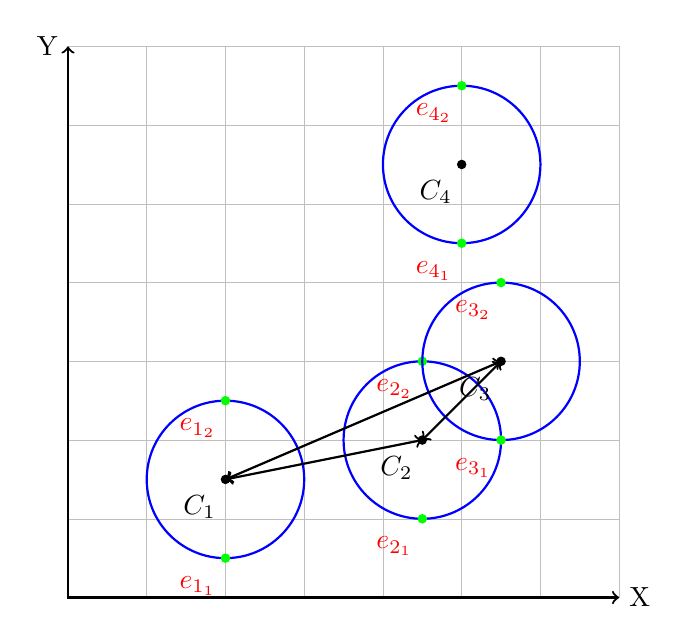
\begin{tikzpicture}[scale=1]
      % grid
      \draw[very thin,color=lightgray] (0,0) grid (7,7);
      \draw [<->,thick] (0,7) node (yaxis) [left] {Y} |- (7,0) node (xaxis) [right] {X};
      
      % Index, x, y, r
      \def\circle[#1,#2,#3,#4] {
    	% The middlepoint
    	\coordinate (C#1) at (#2,#3);
    	
    	
    	% The point
        \draw[fill,color=black] (C#1) circle (1.5pt) node[left, yshift=-10pt, color=black] {$C_#1$};
        
        % The circle
        \draw[thick,color=blue] (C#1) circle (#4);		
        
        % The eventpoints
        \coordinate (E#1_1) at (#2,#3-#4);
        \coordinate (E#1_2) at (#2,#3+#4);
    	
        \draw[fill, color=green] (E#1_1) circle (1.5pt) node[left, yshift=-10pt, color=red] {$e_{#1_1}$};
        \draw[fill, color=green] (E#1_2) circle (1.5pt) node[left, yshift=-10pt, color=red] {$e_{#1_2}$};
      }
      
      \circle[1,2,1.5,1]
      \circle[2,4.5,2,1]    
      \circle[3,5.5,3,1]
      \circle[4,5,5.5,1]
      

      \draw[thick,<->] (C1) -- (C2);
      \draw[thick,<->] (C1) -- (C3);
      \draw[thick,<->] (C2) -- (C3);


      
    \end{tikzpicture}
  }
  \label{fig:voorbeeld_2}
  \caption{Nagekeken cirkels bij algoritme 2}
\end{figure}

\subsection{Linearitmisch}
\label{sec:linearitmisch}

\subsubsection{Algoritme}

\begin{algorithm}[H]
  \SetAlgoLined
  \KwIn{een cirkel $c$ met middelpunt $(x, y)$ en straal $r$}
  \KwOut{een interval $I$ corresponderend aan het interval tussen de uiterste $x$-co\"ordinaten van $c$}
  \SetKwProg{Fn}{Procedure}{:}{end}
  \Fn{interval($c$)}{
    $x_1 \leftarrow x - r$\;
    $x_2 \leftarrow x + r$\;
    $I \leftarrow [x_1, x_2]$\;
    \Return{I}
  }
  \caption{Breedte-interval van een cirkel}
\end{algorithm}
\label{algo:interval}

\begin{algorithm}[H]
  \KwIn{een lijst van $n$ cirkels $C$, gegeven door hun middelpunt en straal}
  \KwOut{een verzameling van $S$ snijpunten $R$ van de cirkels in $C$}
  \SetAlgoLined
  \SetKwProg{Fn}{Procedure}{:}{end}
  \Fn{intersections3($C$)}{
    $E \leftarrow \varnothing$\;
    \For{$c \in C$}{
      $E \leftarrow E \cup events(c)$;
    }
    $E \leftarrow sort(E)$\;
    $T, R \leftarrow \varnothing$\;
    \For{$e \in E$}{
      \uIf {e == insert c} {
        \For{$c' \in T$} {
          \If {$interval(c) \cap interval(c') \neq \varnothing$} {
            $R \leftarrow R \cup intersections(c,c')$
          }
        }
        $T \leftarrow T \cup \left\{c\right\}$
      } \ElseIf {e == delete c} {
        $T \leftarrow T \setminus \left\{c\right\} $
      }
    }
    \Return{R}
  }
  \caption{Linearitmische aanpak (imperatief)}
\end{algorithm}
\subsubsection{Correctheidsbewijs}
\subsubsection{Complexiteit}

\begin{figure}[hbpt]
  \centering
    \begin{tikzpicture}[scale=2]
      % grid
      \draw[very thin,color=lightgray] (0,0) grid (7,7);
      \draw [<->,thick] (0,7) node (yaxis) [left] {Y} |- (7,0) node (xaxis) [right] {X};
      
      \indexedcircle[1,2,1.5,1]
      \indexedcircle[2,4.5,2,1]    
      \indexedcircle[3,5.5,3,1]
      \indexedcircle[4,5,5.5,1]

      \draw[thick,color=blue,arrows={Triangle[scale=1]-Triangle[scale=1]},shorten >=9pt,shorten <=9pt] (C2) -- (C3);

    \end{tikzpicture}
  \label{fig:voorbeeld_23}
  \caption{Nagekeken cirkels bij algoritme 3}
\end{figure}